The design concepts for the tracking system at CEPC are similar to the ones studied for ILC~\cite{Adolphsen:2013kya,Behnke:2013lya},
which are required to provide excellent tracking efficiency and precision over a wide range of momenta for charged particles from the 
interaction point as well as from the decay of secondary particles. The tracking system must be built with minimal
material to preserve the momentum resolution and being covered hermetically down to the dip angle of 
$|cos\theta|<0.992$ from the beam pipe. There are two design options for ILC detectors, the large TPC+Silicon detector (ILD) and 
the compact full-silicon detector (SID), with very different approaches to achieve the same performances. 
The full-silicon tracker offers a well known technology that provides excellent space point resolution and granularity to 
cope track separation in dense jets and hits from the high luminosity beam related background. The drawbacks include the 
relative high materia density within the tracking system, less redundancy, and limited dE/dx measurements. 
Nevertheless, the purpose of this study is to demonstrate that the full-silicon tracking concept is a viable option for CEPC.

For designing a full-silicon tracker, we use the same detector boundary conditions considered in the CEPC v\_4
detector, which are summarized in the following,
\begin{itemize}
 \item the solenoid B field is set to 3~Tesla,
 \item the tracking envolope consists of a cylinder with a radius of 1.83~m and a length of 4.6~m,
 \item the tracker covers down to 7.25 degree from the beam pipe,
 \item the Be beam pipe has a radius of 1.45~cm and 14~cm long.
\end{itemize}

\subsection{Full silicon tracker layout} 
The ILD-like detector relies on a mixture of Time Projection Chamber (TPC) and silicon tracking system. However, the 
tracker could be converted using full silicon if the TPC is replaced with additional silicon stereo-strip layers (SIT) 
in the central region with disks of silicon stereo-strip detectors (FTD) on each side. 
In this design, the outer tracking system consists of a full-silicon tracker arranged as a set of six nested SIT layers in the central 
region with five FTD strip endcap disks on each side as shown in Fig.~\ref{fig:fullsigeom}. Details for design of 
SIT and FTD detectors can be found in the discussion of CEPC-ILD design~\cite{cepcILD} and
 we will use the same module design to build a full silicon detector as CEPC-SID. The pixel vertex detector (VTX) is kept the same as 
in CEPC v\_4.  
     
This new proposed tracking system provides at least 11 precisely measured points for all tracks down to a polar angle of about 15 degree and 
at least 7 measured points down to a polar angle of about 7.25 degree, as shown in Fig.~\ref{fig:fullnhit}. With three double pixel layers 
and forward disks covering a wide of polar angle, they are capable of providing excellent tracking on their own. 
The outer tracker adds additional track-finding constrains at large radii where hit density is low while improving the momentum 
measurement over a large level arm with excellent hit resolution in the transverse plane.

Alternatively, we could optimize the design of ILC-SID detector for CEPC by enlarging the outer silicon strip layers
to fulfil the space up to a radius of 1.83~m and z at $\pm$ 2.3~m in order to achieve comparable momentum resolution using
a lower solenoid B filed of 3~Tesla as shown in Fig~\ref{fig:fullsigeom}. The pixel detectors again are kept the same 
as in the ILC-SID design.  We will label this option as ``SIDB'', which provides an independent cross check on the tracking performance
using a full-silicon tracker. The number of expected hits on the track from SIDB is also shown in Fig.~\ref{fig:fullnhit}.  

Table~\ref{tab:fullsistrips} summarizes the geometry parameters of the proposed outer strip silicon trackers for CEPC between two full silicon 
options.

\begin{figure}[hbtp]
\begin{center}
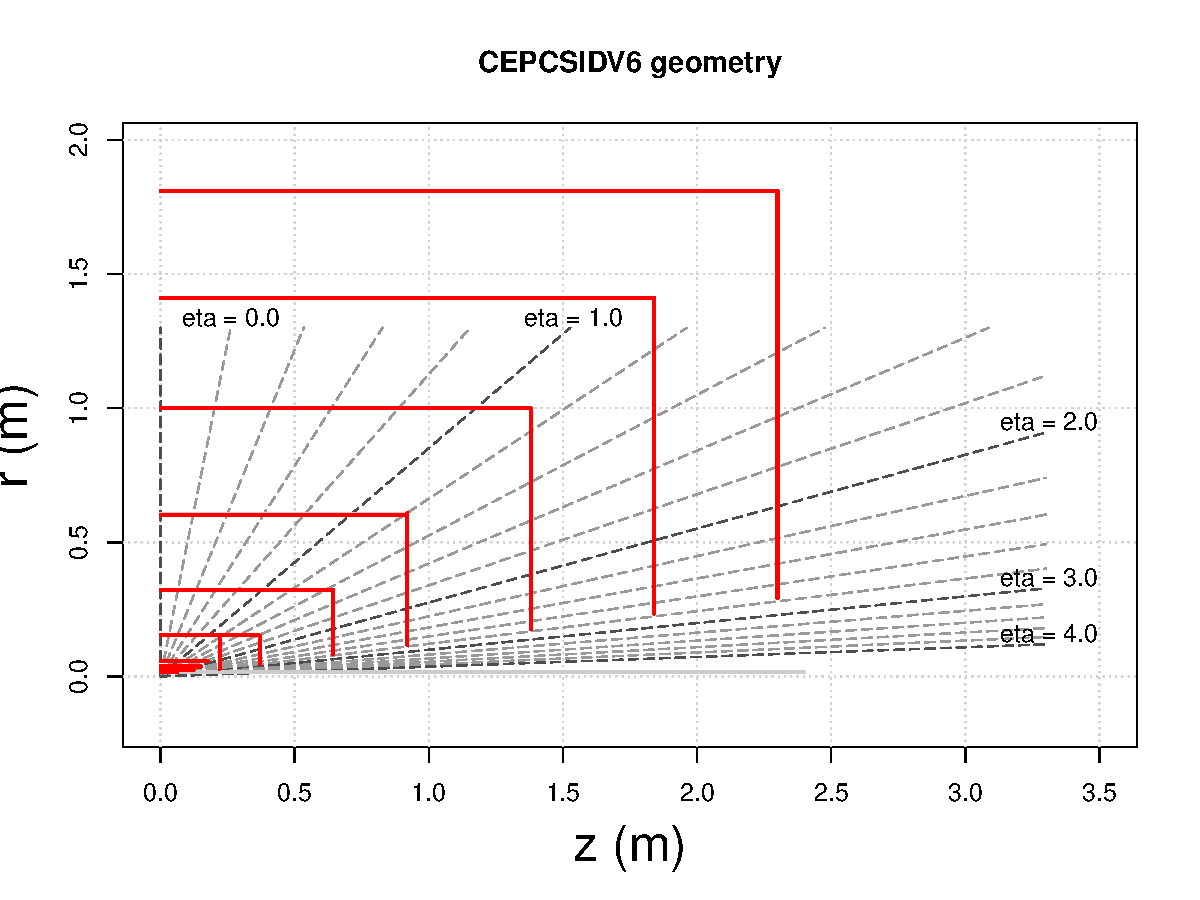
\includegraphics[width=0.32\textheight,keepaspectratio]{Figures/TrackingSystem/FullSilicon/Step1_CEPCSIDV6__geom_R.pdf}
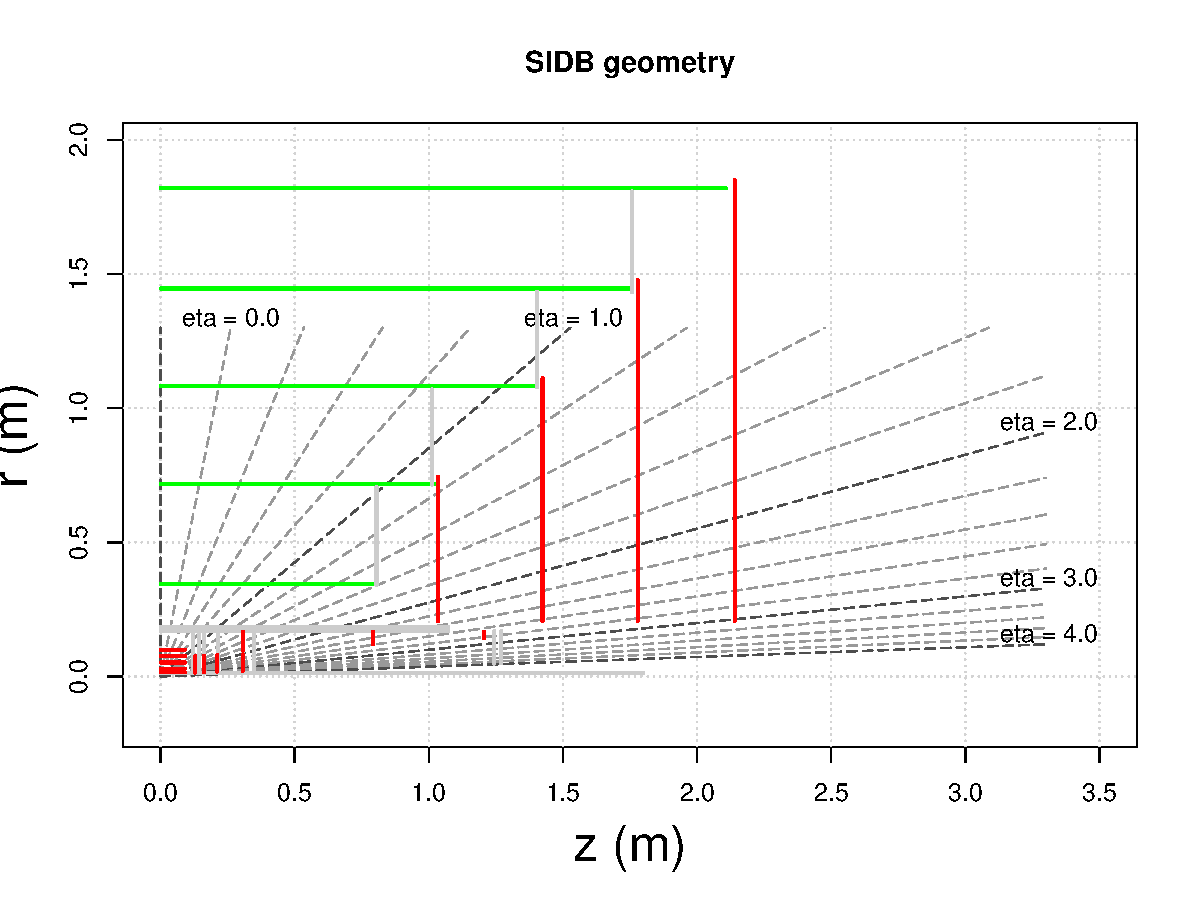
\includegraphics[width=0.32\textheight,keepaspectratio]{Figures/TrackingSystem/FullSilicon/Step1_SIDBig__geom_R.pdf}
\caption{The R-Z view of the full silicon tracker proposed for CEPC (left) and the enlarged version of SID design (right).\label{fig:fullsigeom}}
\end{center}
\end{figure}

\begin{figure}[hbtp]
\begin{center}
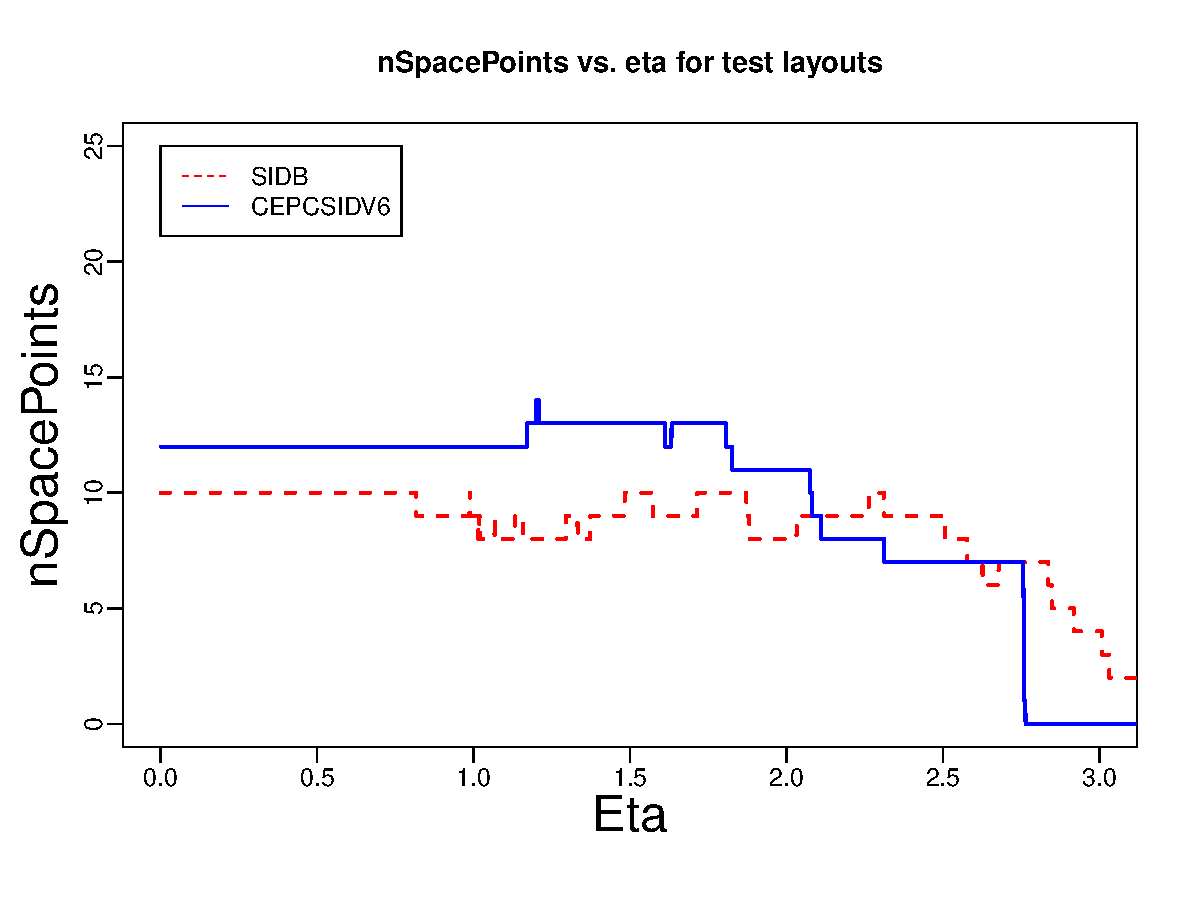
\includegraphics[width=0.45\textheight,keepaspectratio]{Figures/TrackingSystem/FullSilicon/Overlay_nHvsetaZ_R.pdf}
\caption{The number of expected hits are shown as function of track pesuro-rapadity.\label{fig:fullnhit}}
\end{center}
\end{figure}

\begin{table}[htb]
\caption{ The proposed geometry parameters for the outer strip barrel layers and disks,  where D and S stand for 
double and single-strip layer.}
\begin{center}
\begin{tabular}{|c|c|c|c|c|c|c|c|c|} \hline\hline
        & \multicolumn{4}{|c|}{CEPC-SID}          & \multicolumn{4}{|c|}{SIDB} \\ \hline 
Barrel  & \multicolumn{2}{|c|}{R (m)} & $\pm$z (m) & Type &  \multicolumn{2}{|c|}{R (m)} & $\pm$z (m) & Type  \\ \hline 
layer 0 & \multicolumn{2}{|c|}{0.153} & 0.368 & D  & \multicolumn{2}{|c|}{0.344} & 0.793 & S  \\  
layer 1 & \multicolumn{2}{|c|}{0.321} & 0.644 & D  & \multicolumn{2}{|c|}{0.718} & 1.029 & S  \\ 
layer 2 & \multicolumn{2}{|c|}{0.603} & 0.920 & D  & \multicolumn{2}{|c|}{1.082} & 1.391 & S  \\ 
layer 3 & \multicolumn{2}{|c|}{1.000} & 1.380 & D  & \multicolumn{2}{|c|}{1.446} & 1.746 & S  \\
layer 4 & \multicolumn{2}{|c|}{1.410} & 1.840 & D  & \multicolumn{2}{|c|}{1.820} & 2.107 & S  \\\hline 
layer 5 & \multicolumn{2}{|c|}{1.811} & 2.300 & D  & \multicolumn{4}{|c|}{} \\ \hline 
Endcap  & $R_{in}$ (m) & $R_{out}$ (m) & $\pm$z (m) & Type & $R_{in}$ (m) & $R_{out}$ (m) & $\pm$z (m) & Type \\ \hline 
Disk 0  & 0.082 & 0.321 & 0.644 & D & 0.207 & 0.744 & 1.034 & D \\
Disk 1  & 0.117 & 0.610 & 0.920 & D & 0.207 & 1.111 & 1.424 & D \\
Disk 2  & 0.176 & 1.000 & 1.380 & D & 0.207 & 1.477 & 1.779 & D \\
Disk 3  & 0.234 & 1.410 & 1.840 & D & 0.207 & 1.852 & 2.140 & D \\ \hline
Disk 4  & 0.293 & 1.811 & 2.300 & D & \multicolumn{4}{|c|}{} \\ \hline
\hline\hline
\end{tabular}
\end{center}
\label{tab:fullsistrips}
\end{table}

\subsection{Toy simulation} 
For each layout, we use a toy simulation (Idres) to calculate the expected tracking resolution as
function of track momentum for a given incident angle $\theta$, in which the effect of multiple
scattering due to the materia are taken into account correctly. Idres was developed by the ATLAS experiment~\cite{Calace:2015idres}. 
The results are also cross checked using LDT program~\cite{Regler:2008ldt}, which gives a consistent result.

The coverage of the full-silicon tracking system is shown in Fig.~\ref{fig:fullnhit} as function of track pesudo-rapidity. 
At least 7 hits are measured for all tracks with 
a polar angle down to about 7.25 degree. The total radiation length for all-silicon tracking systems, including dead material such as readout,
cables and supports, is about 5-7\% for CEPC-SID and 7-10\% for SIDB, respectively.   
   
The expected momentum ($p_T$) and impact parameters (d0, and z0) resolutions are compared as function of track $p_T$ in GeV/c
for tracks with $\theta =$ 85 and 20 degree, respectively, as shown in Fig.~\ref{fig:toyptd0z0}. The z0 resolution is better for CEPC-SID 
than for SIDB due to extra stereo-strip layers while the $p_T$ and d0 resolutions are similar.

\begin{figure}[hbtp]
\begin{center}
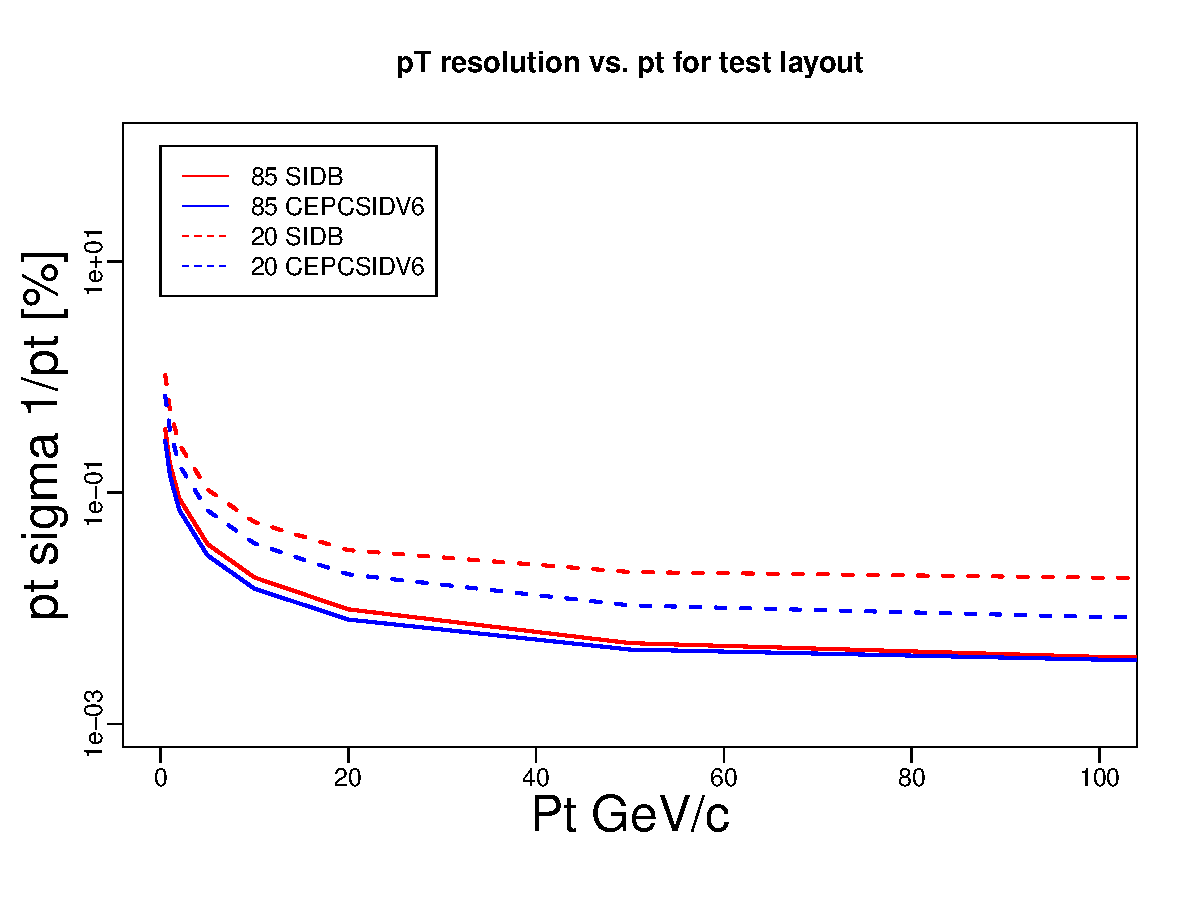
\includegraphics[width=0.32\textheight,keepaspectratio]{Figures/TrackingSystem/FullSilicon/Overlay__ptvsptZ_R.pdf}
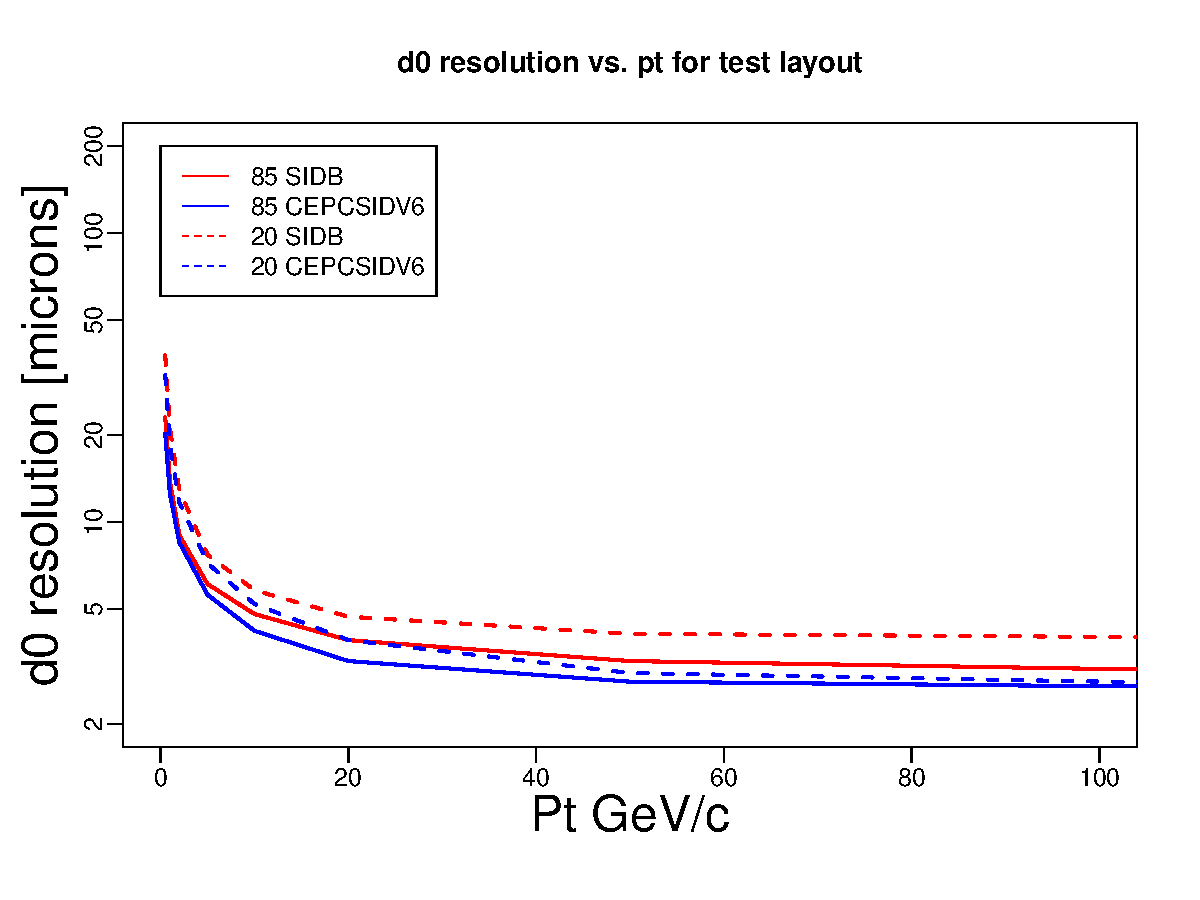
\includegraphics[width=0.32\textheight,keepaspectratio]{Figures/TrackingSystem/FullSilicon/Overlay__d0vsptZ_R.pdf}
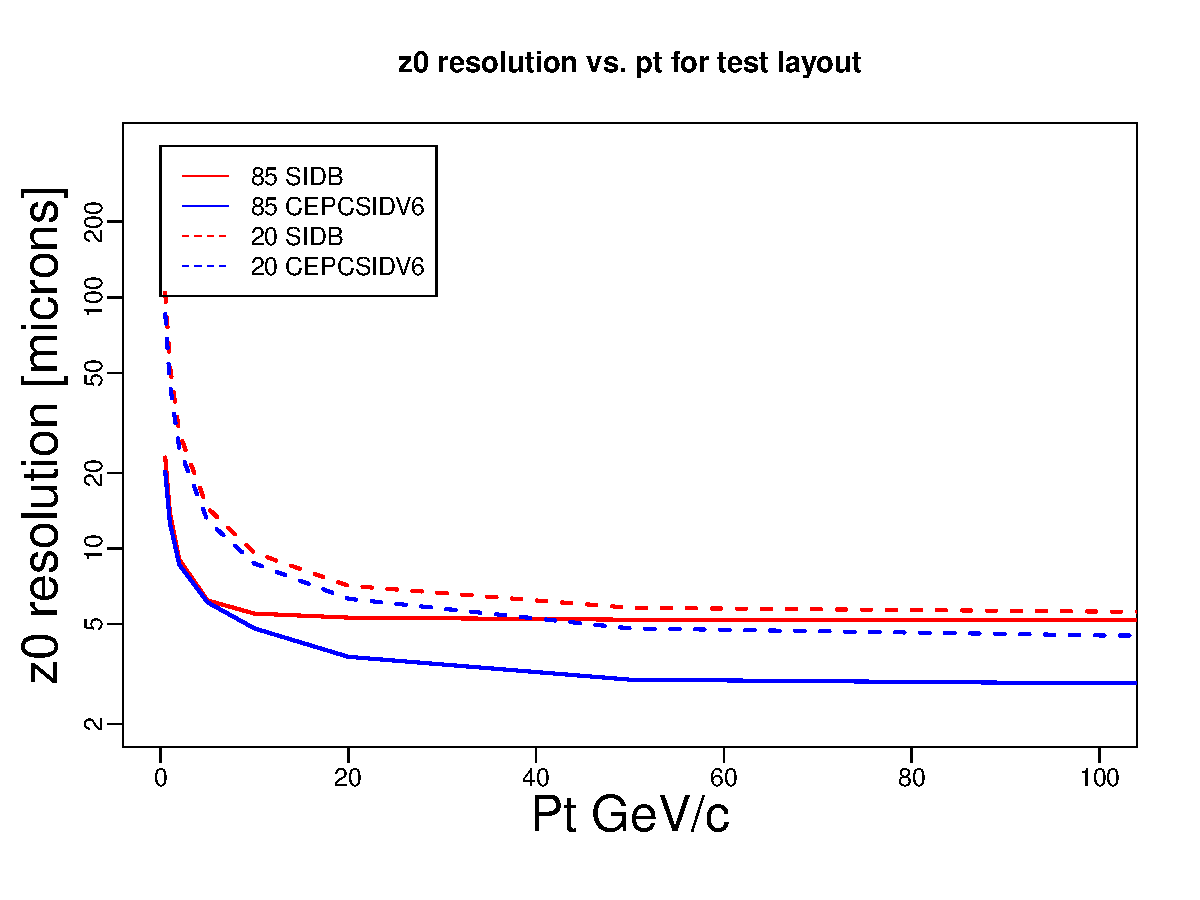
\includegraphics[width=0.32\textheight,keepaspectratio]{Figures/TrackingSystem/FullSilicon/Overlay__z0vsptZ_R.pdf}
\caption{The expected $p_T$, d0, and z0 resolutions from the toy simulation (Idres) are compared as function of track $p_T$ in GeV/c
for tracks with $\theta =$ 85 and 20 degree, respectively. \label{fig:toyptd0z0}}
\end{center}
\end{figure}
   
\subsection{Detector simulation and reconstruction} 
In order to optimize the full silicon tracker detector for CEPC, we generate several benchmark processes that include single muon events, 
$e^+e^- \rightarrow ZH \rightarrow \nu\nu \mu\mu$, and $e^+e^- \rightarrow ZH \rightarrow \nu\nu GG$ (two gluon jets). 
The events are then simulated and reconstructed using 
different detector geometries, which are then used for the tracking performance studies.    

\subsubsection{CEPC-SID detector}
The implement of geometry of full-silicon-tracker is based on a simulation tool Mokka\cite{ilcMokka}. The CEPC group have create a version of 
database cepc\_v4 to build the preliminary design of CEPC detector~\cite{cepcILD}, in which the tracker is composed of VXD, SIT, TPC, SET and FTD. 
In order to implement the full-silicon-tracker, the TPC is considered to be replaced with a new silicon-based strip tracker. Similarly, the new 
silicon tracker is also called as SIT, and the SET is removed at the same time, since the type of the old SIT, the new silicon-based strip tracker 
and the SET are based on the same design. Finally, a full-silicon-tracker including VXD, SIT and FTD is built on the basis of cepc\_v4, as described 
above. 

In order to improve the flexibility of design, a new package of SiTracker is implemented in Mokka which represents the silicon
tracker by planar structure, which consists of a. thin layer of silicon with 150 $\mu m$ thickness and 50 $\mu m$ pitch size. 
For VXD and SIT, they are composed by several layers, and each layer is composed by several ladders, and 
each ladder is divided to several sensors. The SIT layer consist of double silicon layers mounted back to back with a stereo-angle of 7 degree.
For FTD, it is composed by several pixel disks FTD\_PIXEL and several double-side strip 
disks FTD\_STRIP that are composed by petals. The strip FTD disk has two sensitive silicon sub-layers on each side with a stereo-angle of 5 degree.
The number of ladders/petals, the size and position of layers, and the sub-structure of layers can be modified easily in input file as 
globalModelParameter. In future, a XML structure is considered as the method to input parameters.

The lcio format is used to output the simulated signals from the full-silicon-tracker, same as other 
sub-detector system~\cite{lcsim}. The digitization and clustering are done 
in reconstruction process. In the default version, a smearing technology based on truth information 
is used as a simple digitization and clustering, which is used for this study. 
Recently, a new digitization for silicon-based detector has been developed. It first finds out the pixel which the hit is located, and uses the 
center of the pixel or strip as the new position for the hit. And then those hits in same pixel or neighnoring will be merged into single hit.

The silicon tracking algorithm is the same one used by CEPC-ILD~\cite{cepcILD}, which are steered by a set of strategies.
Each strategy represents a set of layers in the detector and tries to find combinations of hits that forms a helix within these layers.
The algorithm starts by looking for a track seed by any combination of three hits that fufils a helix fit. Once found, the track seed is extended
by successively adding more hits that are consistent with the extrapolation of the seed helix.
If fewer than the minimum required number of hits are found, the track candidate is discarded. If the tracks found in different strategies share
more than one hit, only the track with the best fit is kept based on the $\chi^2$ per degree of freedom and the number of hits on the track.
  
\subsubsection{Optimized SID detector}
For the SiD detector optimized for CEPC (or SIDB), events were simulated and reconstructed
using a software developed for the International Linear Collider (ILC)~\cite{Adolphsen:2013kya,Behnke:2013lya}, but
re-worked for the HepSim project \cite{Chekanov:2016sme,Chekanov:2016ppq}.
The response of the SiD detector to physics events
is simulated using the ``Simulator for the Linear Collider'' (SLIC) 5.0  software~\cite{Graf:2006ei}
interfaced with the {\sc Geant4} 10.3p1 program~\cite{Allison2016186}.
The track reconstruction  was performed with the {\sc LCSim} 4.0 package  \cite{lcsim} using
the ``seed tracker'' algorithm as for the SiD detector simulation.
Track candidates with at  least six hits in the silicon pixel and microstrip layers were considered.
Only tracks with a minimum transverse momentum ($p_T$) of $100$~MeV were accepted.
The track-fitting was performed with the following requirements; maximum distance of closest approach (DCA) is $|DCA|<6$~mm, $|z_0|<10$~mm,
and fit $\chi^2 < 10$. The reconstruction includes particle-flow algorithms (PFA)
which enable  identification and reconstruction of individual particles.
The PFA objects can be reconstructed using the software algorithms implemented in
the {\sc pandora} package~\cite{Charles:2009ta,Marshall:2013bda}.

The geometry of SIDB detector is implemented using the compact XML geometry description, which can load and built
at runtime. The main changes over the ILC-SID detector include the reduced B-field from
5~Tesla to 3~Tesla. The outer tracker is scaled up by a factor of about 1.44 to the radius of
1.83~m and $z$ of $\pm$ 2.3~m. The  silicon module sizes were appropriately scaled.
The first inner layer of the barrel vertex detector was positioned at 15~mm, just outside of the beam pipe.
The outer barrel layer of the silicon vertex detector was moved to 100.3~mm (vs 59~mm for the SiD detector), while
other barrel layers are equally spaced. The forward disks, together with the support structures,
were appropriately scaled in $z$ by a factor 1.37.

As for the SiD detector, the barrel tracker consists of five layers of  silicon sensors with 50~$\mu$m  pitch.
The forward tracker has four disks of silicon sensors.
The silicon pixel detector had 20~$\mu$m pitch,  consisting of five layers in the barrel and six disks in the
forward region. The hadronic and  electromagnetic calorimeters, as well as the muon detector,
were optimized for CEPC physics as described in \cite{Chekanov:2016efe}.

\subsection{Tracking performance} 
After the detector simulation and reconstruction, the tracking performances are  measured in terms of efficiencies, 
fake rates, momentum resolution, and the impact parameter resolutions using single muons or $e^+e^- \rightarrow ZH$ events. 
The tracking efficiency is defined as a fraction of stable charged particles that can be matched to well reconstructed tracks. 
The stable particles are defined as those charged particles with $p_T>$1 GeV/c in the detector fiducial region ( $9<\theta<170$ degree), 
originated from the interaction point, and lived long enough to reach the calorimeter. A well reconstructed 
track is defined as sharing more than 50\% of its assigned silicon hits originating from a single particle (truth hits). 
We define a truth hit fraction as ratio of truth hits over total assigned hits of the track using silicon hits only.  A poorly reconstructed track is 
defined to have the truth hit fraction less than 50\%. The fake rate is defined as the fraction of poorly reconstructed tracks out of 
total reconstructed tracks, but this requires a realistic detector simulation, which we are not there yet. 
The tracking performance in the CEPC (v\_4) detector is also shown as the reference.  
    
\subsubsection{Single muon particle} 

Figure~\ref{fig:fullsieff} shows the tracking efficiency for single muons in CEPC-SID  as function of $p_T$. 
The tracking efficiency is close to 100\% at high $p_T$ and slightly lower at small $p_T$. The trend is the same for CEPC v\_4 , which indicate both 
trackers are capable of finding tracks efficiently in the detector fiducial region. 

\begin{figure}[hbtp]
\begin{center}
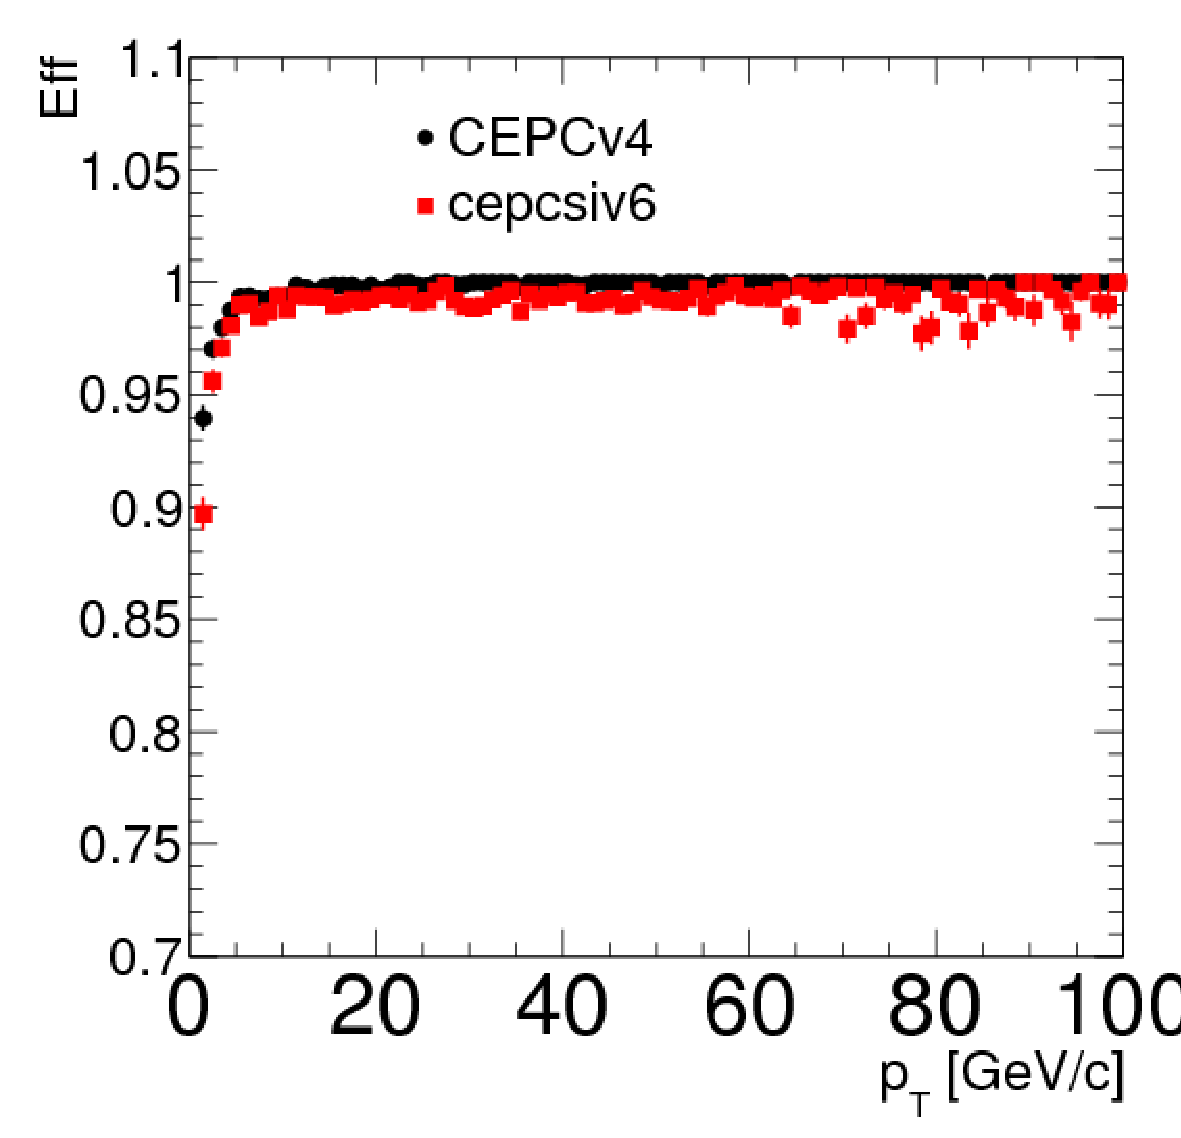
\includegraphics[width=0.45\textheight,keepaspectratio]{Figures/TrackingSystem/FullSilicon/Plot_muon_Eff_Pt.pdf}
\caption{The tracking efficiencies are measured as function of $p_T$ for single muons using CEPC v\_4 and 
CEPC-SID detetcors. \label{fig:fullsieff}}
\end{center}
\end{figure}

The number of silicon hits found on the track and the fraction of truth hits  are shown in Fig.~\ref{fig:fullsinhit} where the hit 
purity is reached more than 90\% for both detectors. 

\begin{figure}[hbtp]
\begin{center}
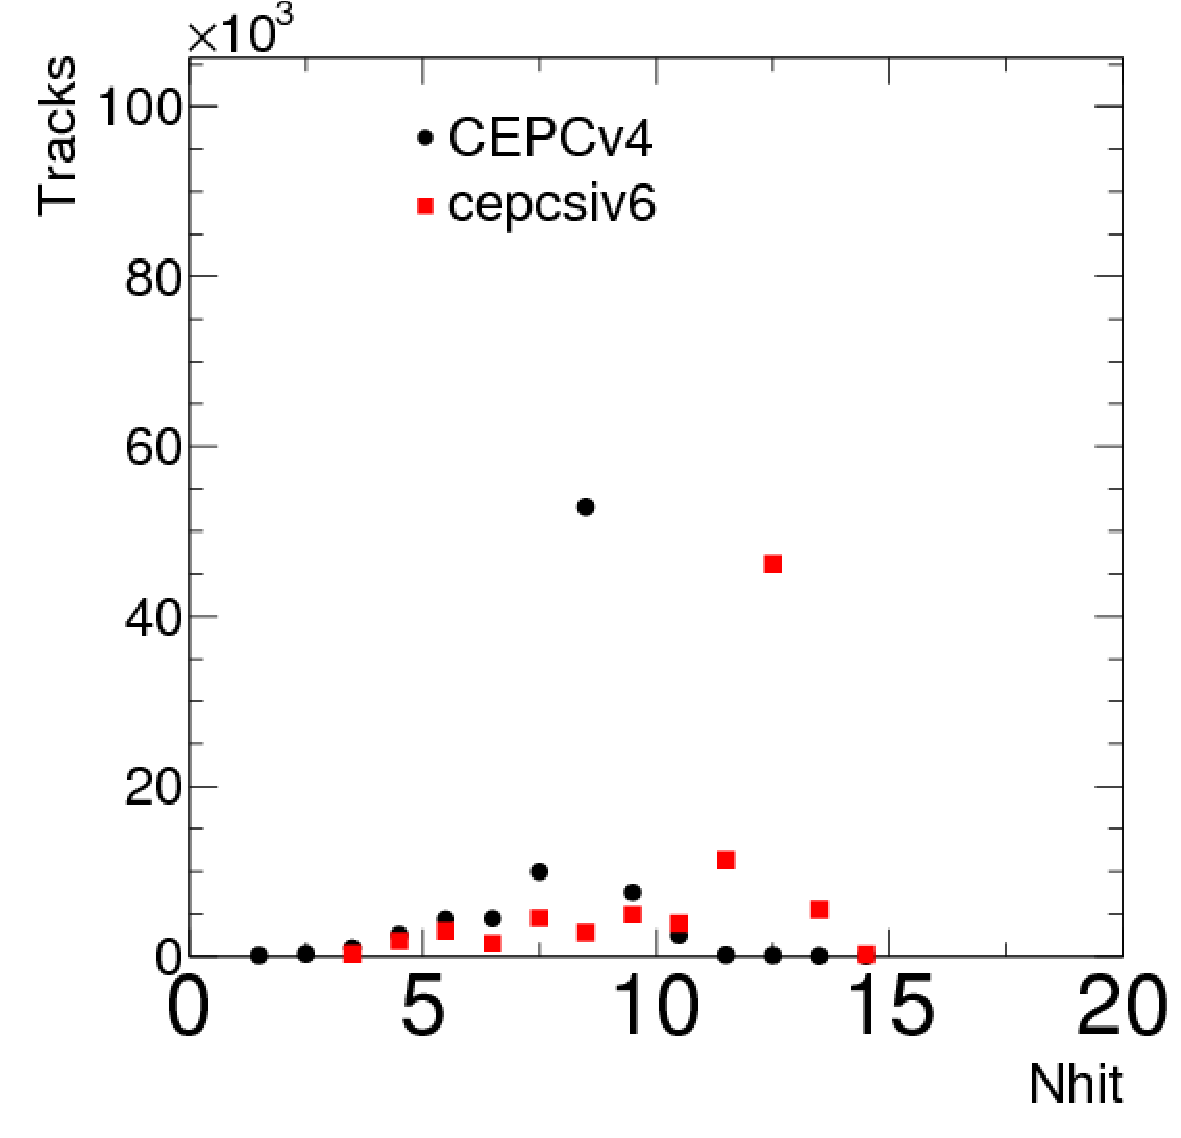
\includegraphics[width=0.45\textheight,keepaspectratio]{Figures/TrackingSystem/FullSilicon/Plot_muon_Nhit.pdf}
\caption{The distributions are shown for the number of silicon hits on the track (left) and the hit purity on (right).\label{fig:fullsinhit}}
\end{center}
\end{figure}


Since the track resolution depends on the track angle $\theta$, we divide the tracks in the barrel 
region with $40<\theta<140$ degree and in the endcap region with $7.25<\theta<40$ degree or $140<\theta<172.75$ degree. 
Figure~\ref{fig:detptd0z0} shows the track resolutions of $p_T$, d0, and z0 as function of track $p_T$ in the barrel and endcap region. 
The resolutions for the low momentum tracks seem slightly better in the CEPC v\_4 detector (TPC+Silicon) than an alternative full silicon tracker due 
to extra materia in the detector while they are compatible at the high $p_T$. 
The resolutions from the SIDB detector are also included in the comparision, which has a compatible momentum resolution 
while the d0 and z0 are slightly worse.

\begin{figure}[hbtp]
\begin{center}
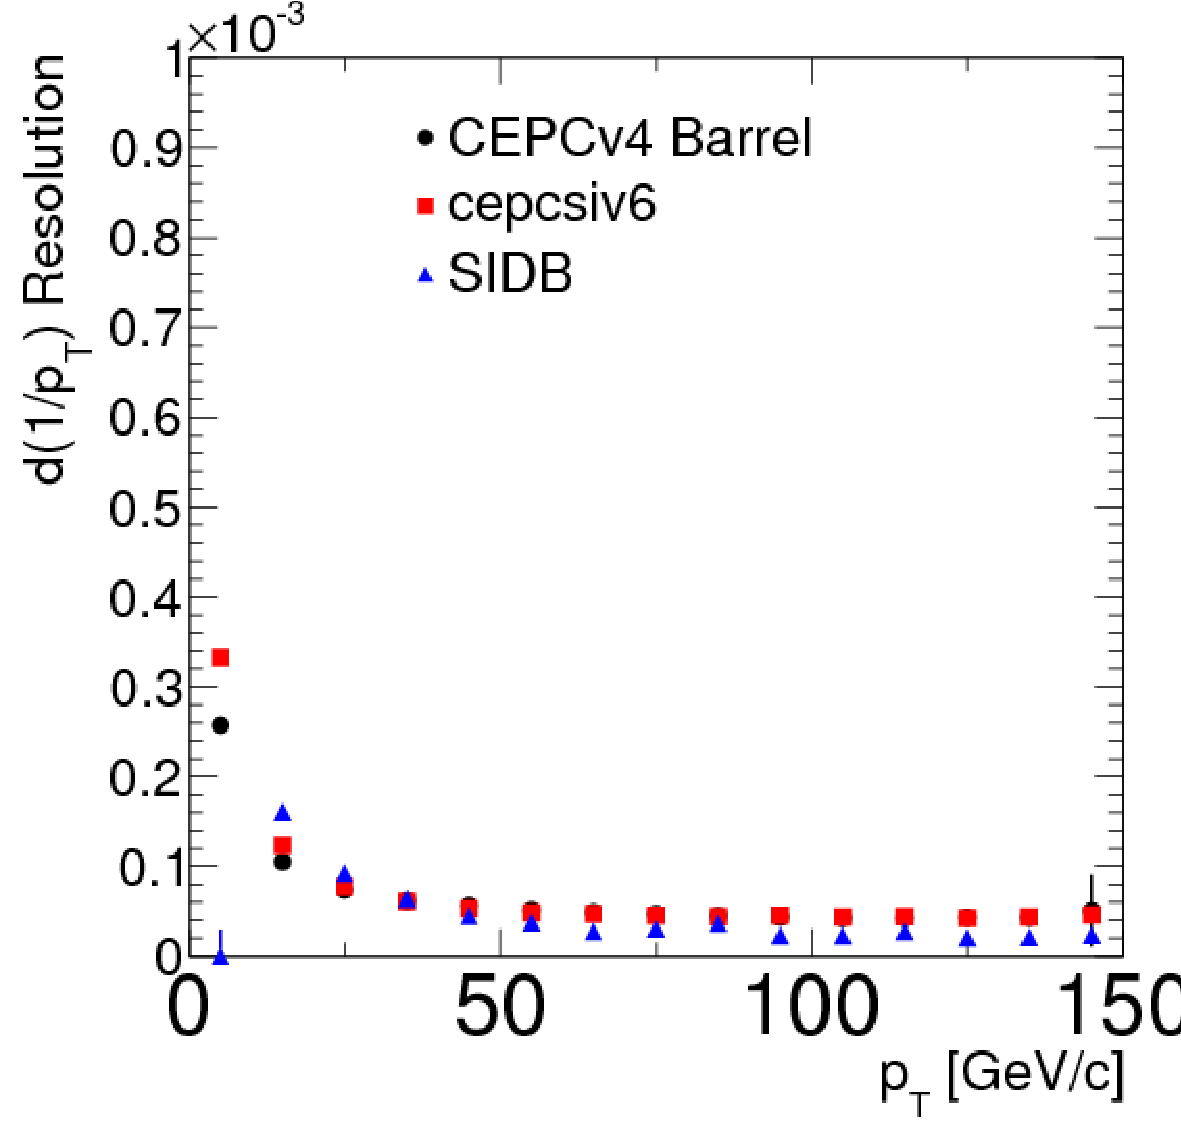
\includegraphics[width=0.25\textheight,keepaspectratio]{Figures/TrackingSystem/FullSilicon/Plot_muon_Pt_PtBarrel.pdf}
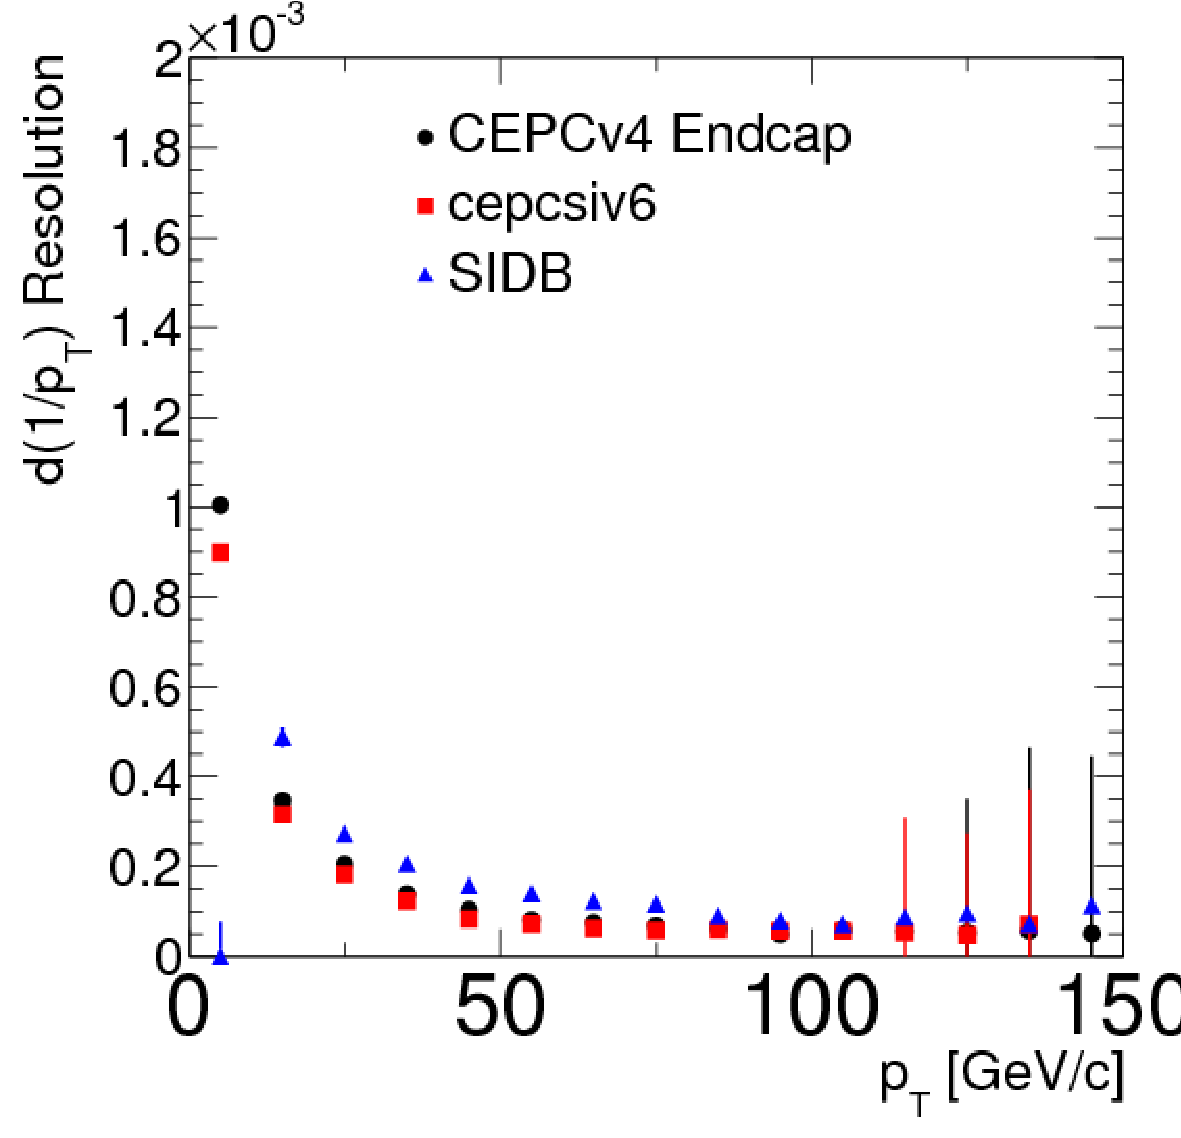
\includegraphics[width=0.25\textheight,keepaspectratio]{Figures/TrackingSystem/FullSilicon/Plot_muon_Pt_PtEndcap.pdf}
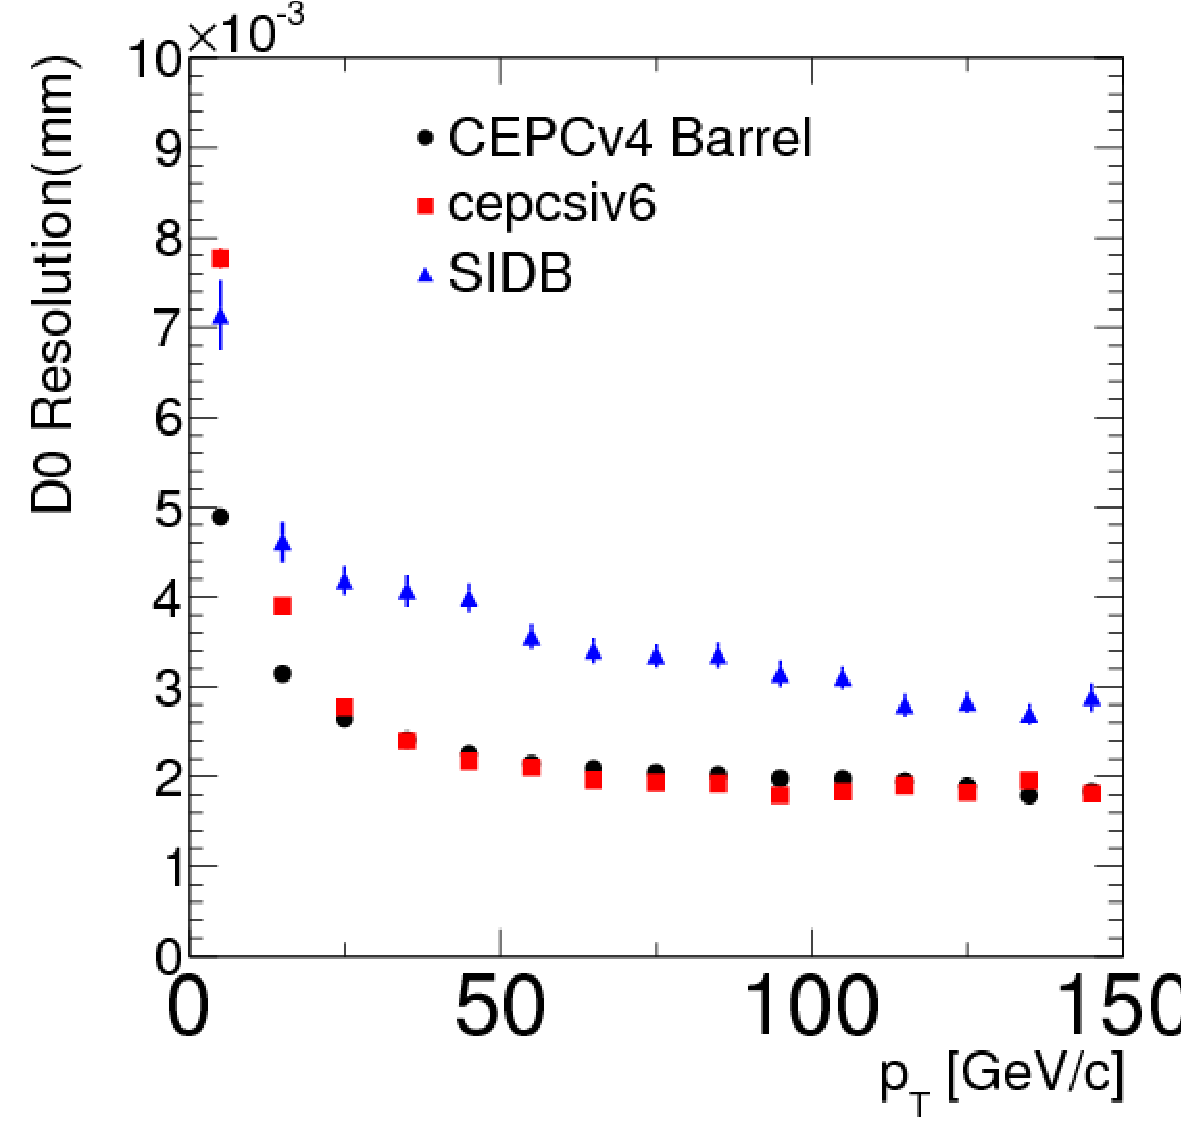
\includegraphics[width=0.25\textheight,keepaspectratio]{Figures/TrackingSystem/FullSilicon/Plot_muon_D0_PtBarrel.pdf}
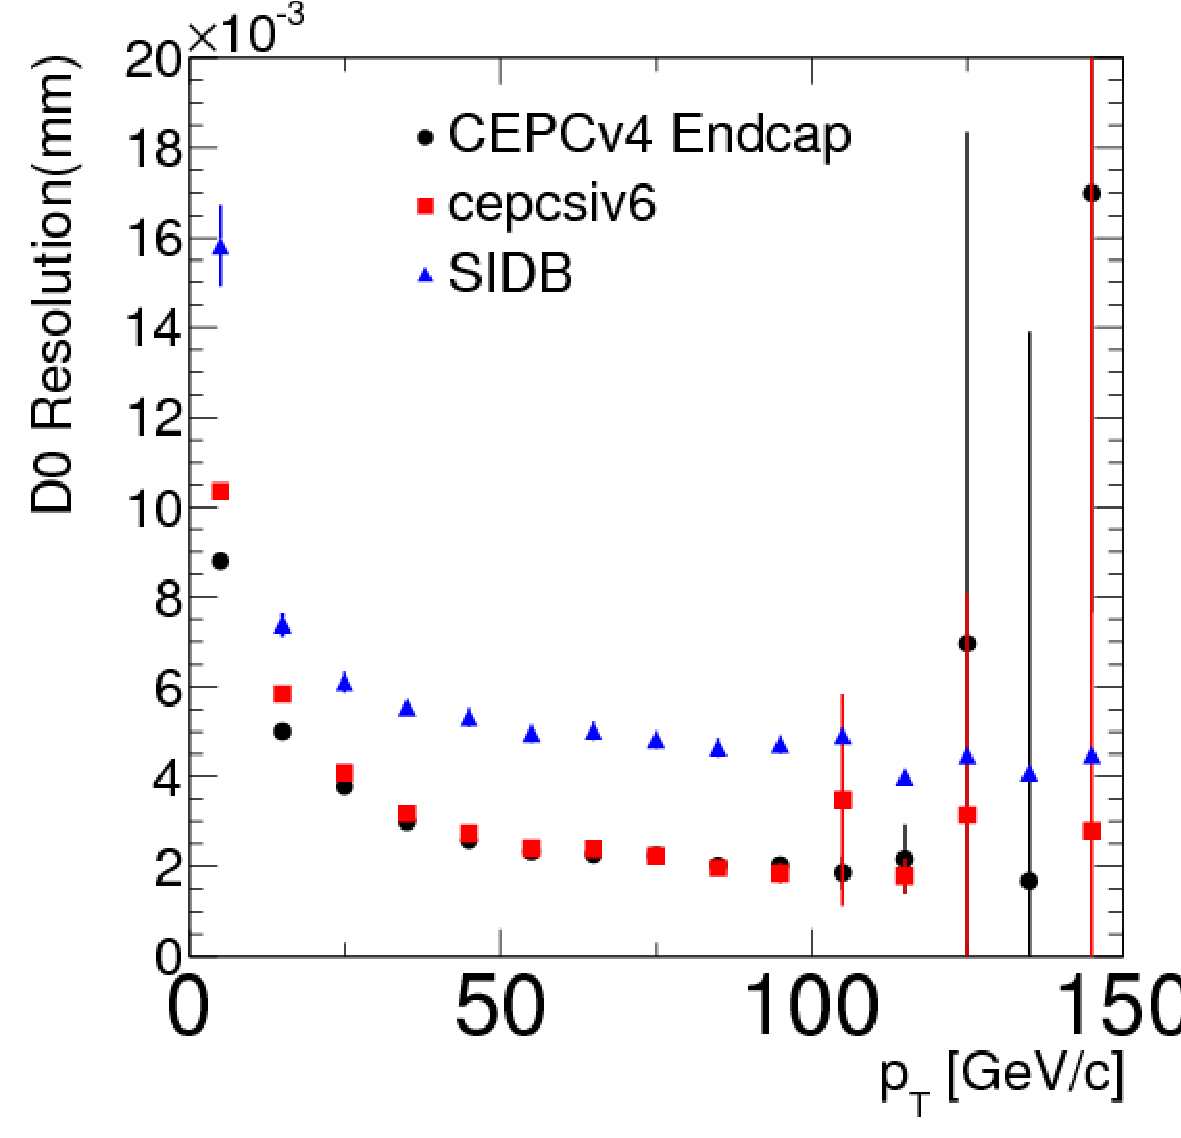
\includegraphics[width=0.25\textheight,keepaspectratio]{Figures/TrackingSystem/FullSilicon/Plot_muon_D0_PtEndcap.pdf}
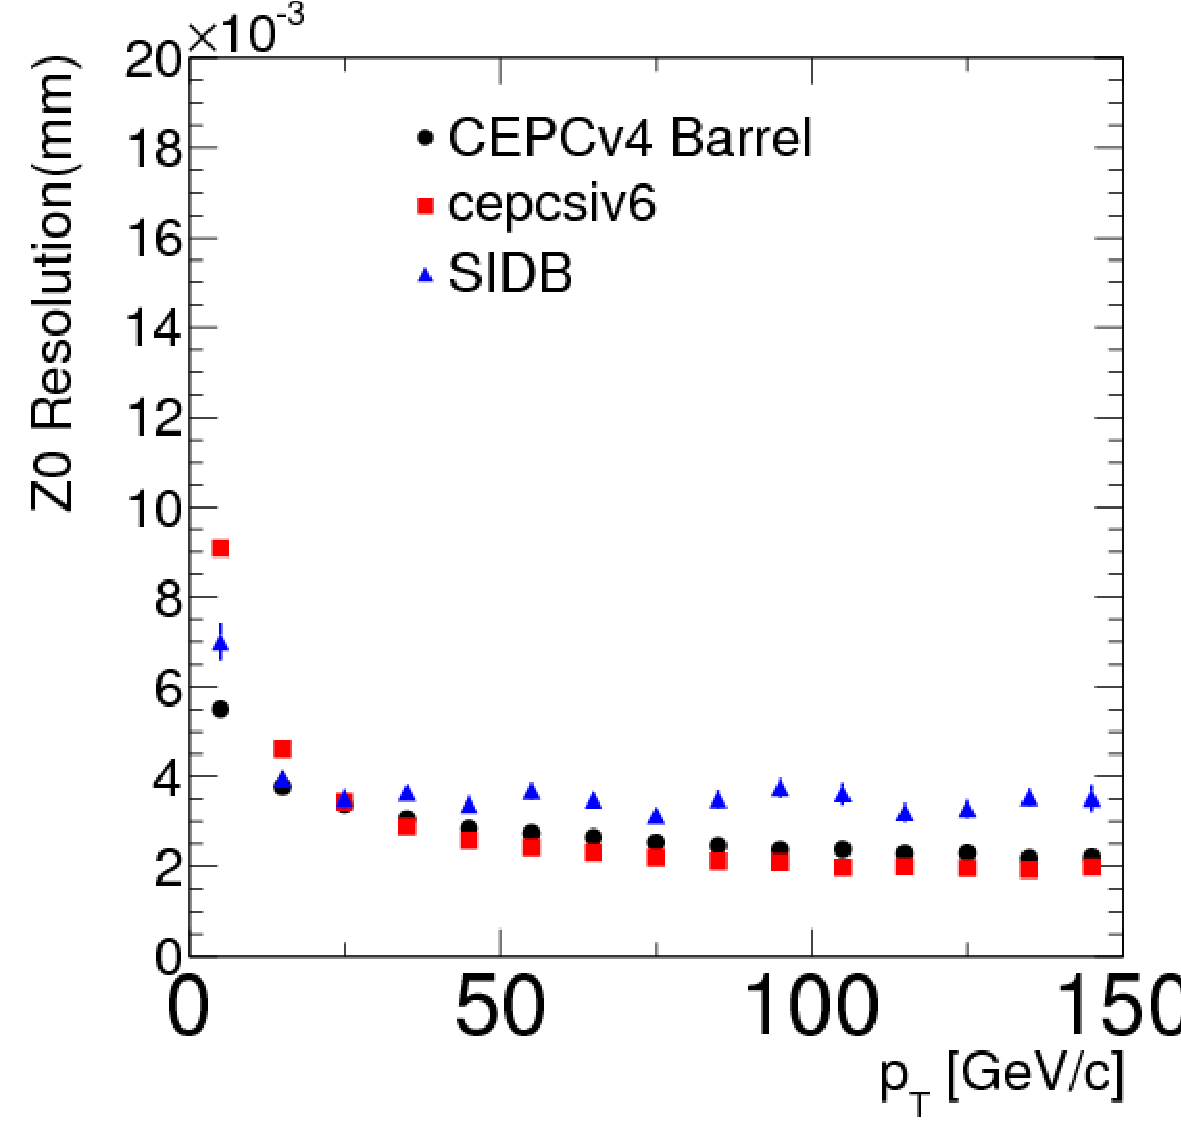
\includegraphics[width=0.25\textheight,keepaspectratio]{Figures/TrackingSystem/FullSilicon/Plot_muon_Z0_PtBarrel.pdf}
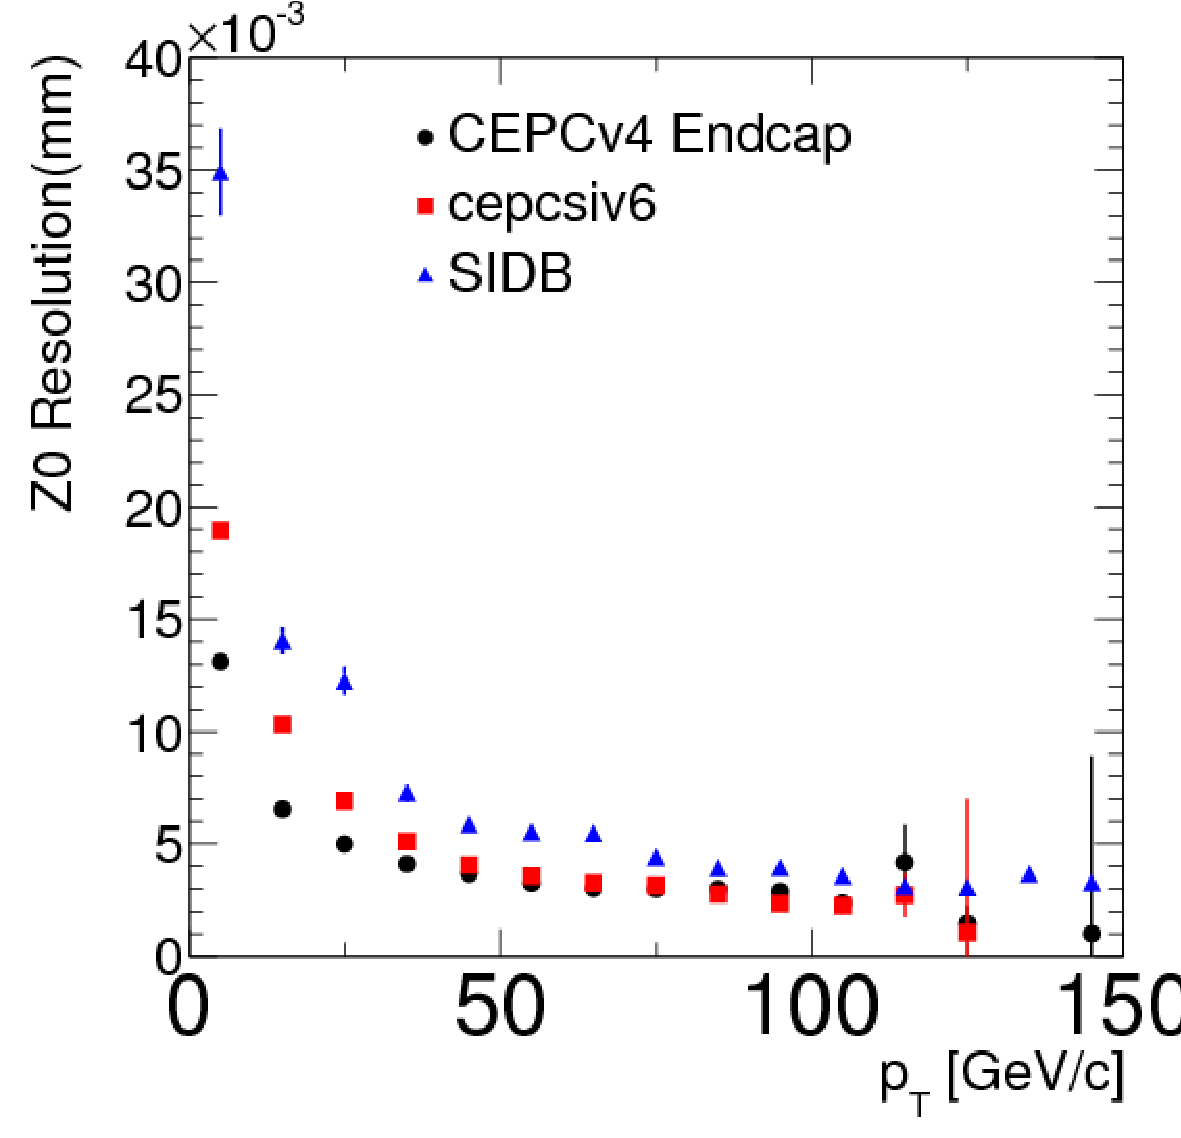
\includegraphics[width=0.25\textheight,keepaspectratio]{Figures/TrackingSystem/FullSilicon/Plot_muon_Z0_PtEndcap.pdf}
\caption{The tracking $p_T$, d0, and z0 resolutions are measured as function of $p_T$, $\phi$, and $\theta$ using single muons, 
left in the barrel region and right in the endcap region. They are compared between CEPC v\_4 and two full silicon detector concepts.\label{fig:detptd0z0}}
\end{center}
\end{figure}
 
\subsubsection{Di-muon mass resolution} 

Figure~\ref{fig:dimuons} shows the di-muon invariant mass distributions from $ZH\rightarrow \nu\nu \mu\mu$ decay between
different detector configurations. The higgs mass used in CEPC simulation is 125 GeV/c$^2$ while 125.09 GeV is used in the SIDB simulation. 
The di-mass from CEPC-ILD seems shifted by 0.2 GeV from the input Higgs mass of 125 GeV/c$^2$ while other masses from CEPC-SID and SIDB
agree with the expectation. The di-muon mass resolution from CEPC-SID has $\sigma=0.21$ GeV/c$^2$ and seems 20\% and 25\% better 
than ones obtained from CEPC-ILD and SIDB, respectively. 

\begin{figure}[hbtp]
\begin{center}
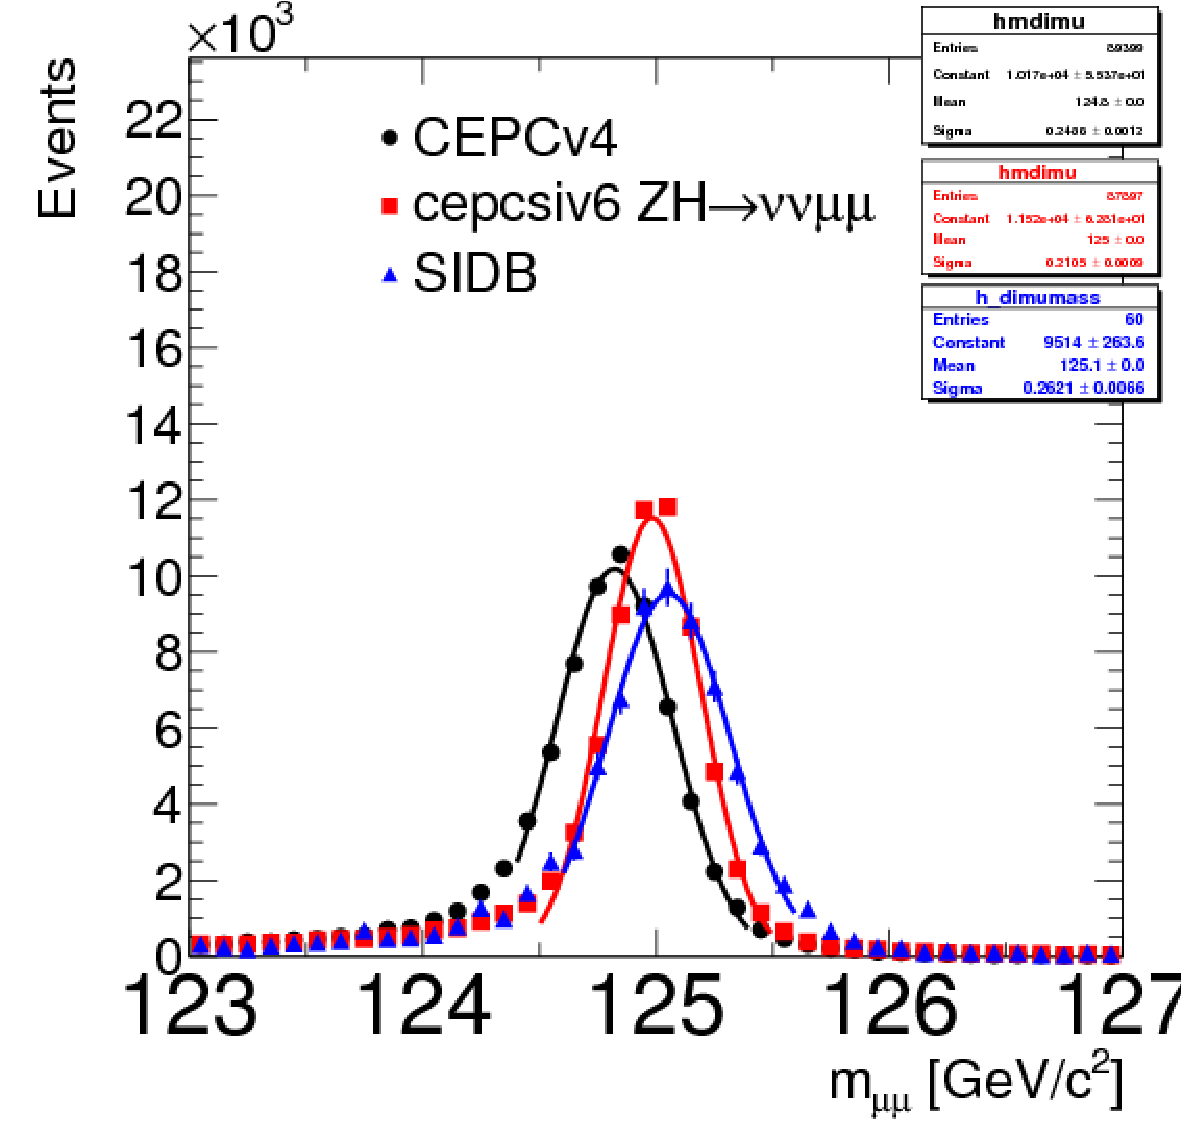
\includegraphics[width=0.45\textheight,keepaspectratio]{Figures/TrackingSystem/FullSilicon/Plot_zhnnmumu_DimuonMass.pdf}
\caption{The di-muon mass distribution is compared from different detectors.\label{fig:dimuons}}
\end{center}
\end{figure}

\subsubsection{Tracking inside the jets} 

In order to study the tracking performance inside the jets, we generated and simulated some Higgs decaying into two gluon jets (GG) in 
$zH\rightarrow \nu\nu GG$ events. Figure~\ref{fig:glgl} shows the tracking efficiency inside the jets as function of track momentum.
The average efficiency of finding tracks inside the jets is about 90\% for CEPC-SID while about 97\% for 
CEPC-ILD due to the excellent tracking in TPC. The full silicon tracking inside the dense of jets is not fully optimized in 
dealing with outliers in the fit, which requires a realistic detector simulation and clustering. The work is in progress to improve
the tracking inside the jets.  
 
\begin{figure}[hbtp]
\begin{center}
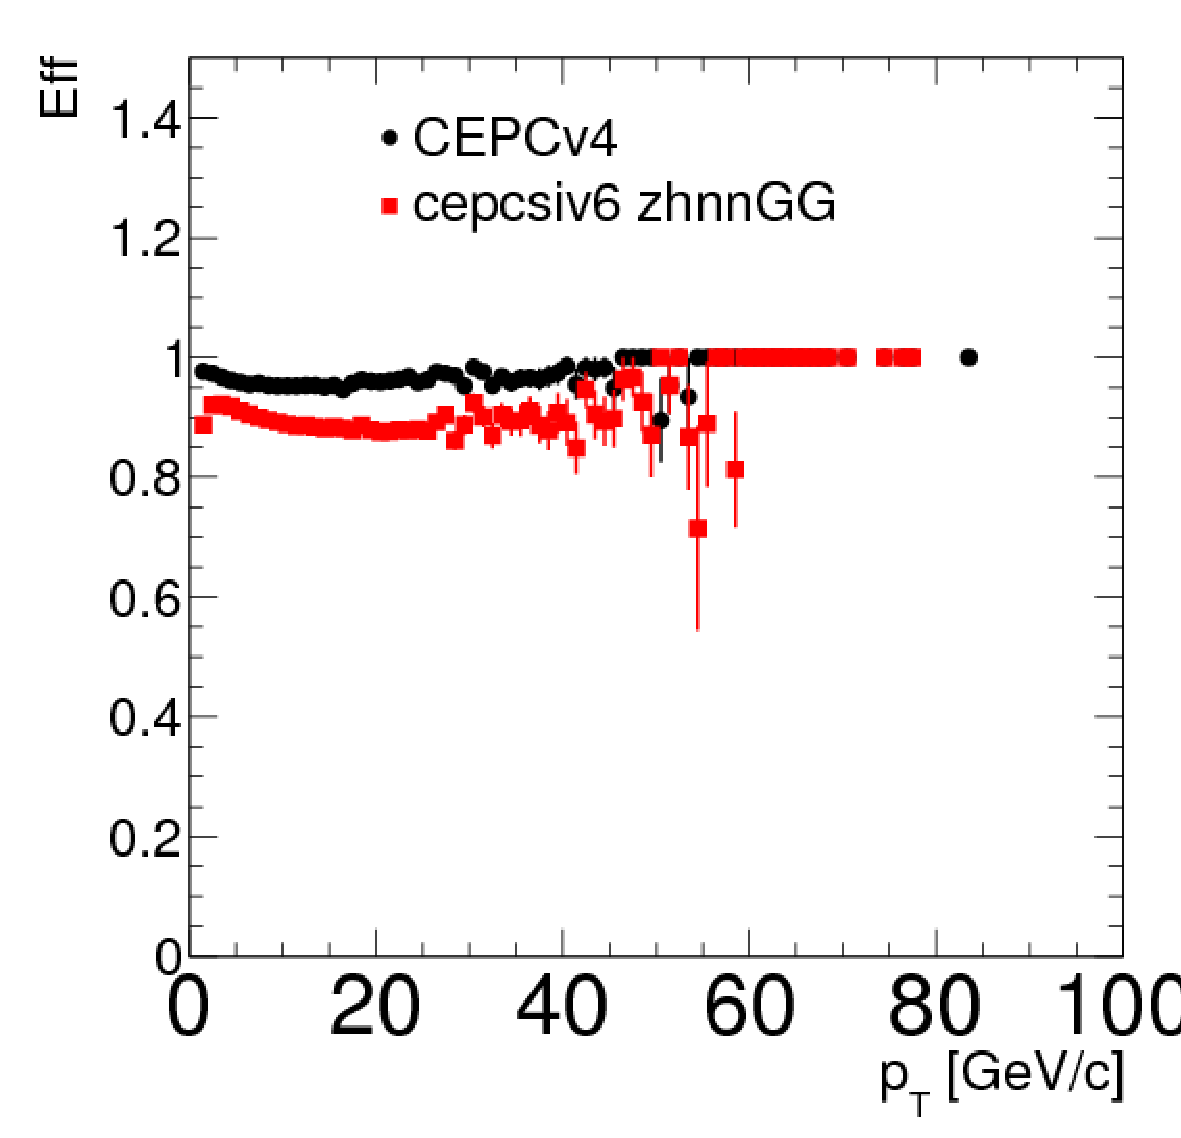
\includegraphics[width=0.45\textheight,keepaspectratio]{Figures/TrackingSystem/FullSilicon/Plot_zhnnGG_Eff_Pt.pdf}
\caption{The tracking efficiencies for the stable particles inside the gluon jets as 
function of track $p_T$ with CEPC v\_4 and CEPCSID.\label{fig:glgl}}
\end{center}
\end{figure}

\subsection{Conclusion} 
  We present a preliminary study of full silicon tracker option as an alternative design for CEPC tracking.
  Two approaches are considered for the design: the first is to keep the
  silicon detectors (VXD, SIT, FTD) in the CEPC-ILD detector and replacing TPC with additional silicon detectors,
  the second is to optimize the ILC-SID tracker to fulfil the CEPC tracking volume in order to achive the
  excellent momentum resolution using 3 Tesla B field. The new detector geometry has been implemented in
  the simulation and the track reconstruction has also been adoped for the full silicon tracker.
  The initial study of the tracking performance looks promising. There are still many improvements 
  needed in the simulation and reconstruction in order to explore the full potential of the full-silicon tracker. 

